%!TEX root = ../lections.tex
	Динамические системы с одномерным фазовым пространством – системы
на прямой являются простейшим видом непрерывных динамических систем с
конечномерным фазовым пространством. Сами по себе такие модели
описывают поведение достаточно простых реальных систем. Например,
изменение заряда $q$ в простейшем $RC$-контуре (рис. \ref{fig:2.1}), содержащем конденсатор с сегнетоэлектриком (вещество с нелинейной зависимостью поляризации от приложенного электрического поля).
\begin{figure}[h!]
	\begin{minipage}{0.49\linewidth}
		\centering
		
\includegraphics[]{fig/lect2/1a}
		% \caption{(a)}
	\end{minipage}
	\hfill
	\begin{minipage}{0.49\linewidth}
		\centering
		
\includegraphics[]{fig/lect2/1b}
		% \caption{(b)}
	\end{minipage}
	\caption{(a) ~ $RC$-контур; (b) нелинейная характеристика конденсатора с диэлектриком}
	\label{fig:2.1}
\end{figure}

	
Однако, с методической точки зрения эти системы чрезвычайно важны,
поскольку дают наглядное и ясное представление о базовых идеях и подходах
теории колебаний.
\section{Качественный подход} % (fold)
Во многих случаях качественные (геометрические) представления о
динамике нелинейных систем бывают более полезны, чем даже точное решение
системы. Поясним это на простом примере. Рассмотрим уравнение
\begin{equation}
	\label{eq:2.1}
	\dot x = x- x^2
\end{equation}

Очевидно, что $x=0$ и $x=1$ является решениями \eqref{eq:2.1}. Найдем остальные решения. Считая, что $x\neq 0;\,1$, разделим переменные в \eqref{eq:2.1}
\begin{equation}
	\label{eq:2.2}
	\frac{\dd{x}}{x-x^2}= \dd{t}
\end{equation}
Интегрируя \eqref{eq:2.2}, получаем 
\begin{equation}
	\label{eq:2.3}
	\ln|x| - \ln|1-x|+C=t,		
\end{equation}
где $C=\const$. Рассмотрим решение уравнения \eqref{eq:2.1}, удовлетворяющее начальному условию: $x(0)=x_0,$ где $x_0\neq 0\,1$. Из \eqref{eq:2.3} находим, что этому начальному условию отвечает постоянная
\begin{equation}
	\label{eq:}
	C=\ln|1-x_0| - \ln|x_0|
\end{equation}
и соответствующее решение имеет вид
\begin{equation}
	\label{eq:2.4}
	\ln\abs{\frac{x}{x_0}} - \ln\abs{\frac{1-x}{1-x_0}}=t
\end{equation}
Выражение \eqref{eq:2.4} задает точное решение рассматриваемой задачи. Давайте попробуем получить из \eqref{eq:2.4} ответы на следующие вопросы:
\begin{enumerate}
	\item Пусть $x_0=\frac12$. Как изменяется переменная $x(t)$ при $t>0$ и, в частности, какое предельное значение она принимает при $t \rightarrow +\infty$?
	\item Как ведёт себя $x(t)$ при $t \rightarrow + \infty$ при различных значениях $x_0$?
\end{enumerate}

Конечно, из \eqref{eq:2.4} ответить на эти вопросы можно, но это требует некоторых дополнительных рассуждений и выкладок. Давайте теперь для ответа на эти вопросы привлечем базовое понятие теории колебаний -- фазовое пространство. Для системы \eqref{eq:2.1} фазовым пространством является числовая прямая $\R^1$. Отметим на $\R^1$ значения $x=0$ и $x=1$. В этих точках $\dot x=0$ и, следовательно, эти значения не изменяются во времени. Из \eqref{eq:2.1} легко найти знак $\dot x$ во всех интервалах прямой $\R^1$, определяемых значениями $x=0$ и $x=1$, и тем самым установить направление движения фазовых траекторий. Отсюда, принимая во внимание структуру разбиения фазовой прямой на траектории, легко дать ответы на поставленные вопросы.

\begin{figure}[h!]
	\centering
	
\includegraphics[]{fig/lect2/2}
	\caption{Фазовая прямая системы \eqref{eq:2.1}}
	\label{fig:2.2}
\end{figure}





\begin{enumerate}
	\item Траектория с начальным условием $x_0=\frac12$ при $t \rightarrow + \infty$ асимптотически стремится к значению $x=1$.
	\item Все траектории с начальными условиями $x_0>0$ ($x_0\neq1$) при $t \rightarrow + \infty$ асимптотически стремятся к значению $x=1$ , а при $x_0<0$ переменная $x(t)$ неограниченно убывает, т.е. $x(t) \rightarrow - \infty$. 
\end{enumerate}

Рассмотренный пример показывает, что в фазовом пространстве существуют значения $x$, которые остаются неизменными при любом $t$ -- это так называемые состояния равновесия (см. лекцию \ref{lect1}, раздел \ref{subsubsec:1.2.1}). С теоретической точки зрения любое состояние равновесия представляет собой классический геометрический объект -- точку. В системе \eqref{eq:2.1} к точке $x=1$ траектории системы асимптотически приближаются при $t \rightarrow + \infty$ и поэтому это состояние равновесия логично называть устойчивым, а от точки $x=0$ траектории, наоборот, удаляются при увеличении $t$ и его, поэтому, называют неустойчивым (строгое определение устойчивости состояний равновесия мы дадим позднее).

% subsection качественный_подход (end)

\section{Грубые состояния равновесия} % (fold)
\label{subsec:2.2}

Рассмотрим динамическую систему на прямой общего вида
\begin{equation}
	\label{eq:2.5}
	\dot x = F(x, \vec \mu) =0,
\end{equation}
где $x \in \R^1$, $\vec \mu \in \R^m$ -- вектор параметров. Будем считать, что $F(x)$ -- взаимнооднозначная функция, обеспечивающая выполнение теорем существования и единственности решений. Очевидно, что состояние равновесия системы \eqref{eq:2.5} определяются уравнением
\begin{equation}
	\label{eq:2.6}
	F(x, \vec \mu) =0.
\end{equation}
Пусть $x=x^*(\vec \mu)$ -- одно из решений уравнения \eqref{eq:2.6}. Найдем условия локальной устойчивости состояния равновесия $x^*(\vec \mu)$. Пусть $\xi(t) = x - x^*(\vec \mu)$ -- малое возмущение, тогда из системы \eqref{eq:2.5} имеем
\begin{equation}
	\label{eq:}
	\dot \xi = F(x^*(\vec \mu)+ \xi, \vec \mu) = F(x^*(\vec \mu), \vec \mu) + F^\prime_x (x^*(\vec \mu), \mu) \xi + \dots
\end{equation}
или
\begin{equation}
	\label{eq:2.7}
	\dot \xi = F^\prime_x (x^*(\vec \mu), \mu) \xi + \dots
\end{equation}

Если $F^\prime_x (x^*(\vec \mu), \mu) \neq 0$, то в малой окрестности $x=x^*(\vec \mu)$ в  \eqref{eq:2.7} можно ограничиться лишь линейным слагаемым по $\xi$, т.е. вместо \eqref{eq:2.7} рассмотреть линейное уравнение (эта процедура называется линеаризацией, рамки применения которой мы обсудим позднее) вида
\begin{equation}
	\label{eq:2.8}
	\dot x = \lambda(\vec \mu) \xi, \text{ где } \lambda(\vec \mu) = F^\prime_x (x^*(\vec \mu), \mu).
\end{equation}
Поскольку общее решение уравнения \eqref{eq:2.8} имеет вид
\begin{equation}
	\label{eq:}
	\xi(t) = Ce^{\lambda(\vec \mu)t},
\end{equation}
где $C=\const$, то при условии $\lambda(\vec \mu)<0$ возмещение $\xi(t) \rightarrow 0$ при $t \rightarrow + \infty$ и состояние равновесия $x^*(\vec \mu)$ будет устойчивым, а если $\lambda(\vec \mu) > 0 $, то $\xi(t)$ растут и $x^*(\vec \mu)$ будет неустойчивым. Коэффициент $\lambda (\vec \mu)$ называется ляпуновским характеристическим показателем. Условия устойчивости допускают простую геометрическую интерпретацию. Состояние равновесия $x^*(\vec \mu)$ является локально устойчивым, если производная функции $F(x, \vec \mu)$ по точке $x^*(\mu)$ отрицательная и неустойчиво, если $F^\prime(x^*(\vec \mu), \mu)>0$ (рис. \ref{fig:2.3}) 

\begin{figure}[h!]
	\centering
	\begin{minipage}{0.39\linewidth}
		\centering
		\def\svgwidth{\linewidth}
		\input{fig/fig2_3a.pdf_tex}
		% \caption{(a)}
		\label{fig:2.3a}
	\end{minipage}
	\hfill{}
	\begin{minipage}{0.39\linewidth}
		\centering
		\def\svgwidth{\linewidth}
		\input{fig/fig2_3b.pdf_tex}
		% \caption{(b)}
		\label{fig:2.3b}
	\end{minipage}
	\caption{Поведение функций $F(x, \vec \mu)$ в окрестности точки $x=x^*(\vec \mu)$ в случае устойчивого (а) и неустойчивого (b) состояний равновесия.}
	\label{fig:2.3}
\end{figure}

Ясно, что в обоих случаях малые изменения правой части системы \eqref{eq:2.5} не могут привести к исчезновению и смене устойчивости состояния равновесия $x^*(\vec \mu)$. Следовательно, условие грубости состояний равновесия на прямой имеет вид $\lambda(\vec \mu) \neq 0$, а буфуркационные значения параметров определяются уравнением $\lambda(\vec \mu^*)=0$. Таким образом, динамическая система \eqref{eq:2.5} на прямой будет грубой (структурно устойчивой), если для всех состояний равновесия выполнено условие $\lambda_i (\vec \mu) \neq 0$.

% subsection грубые_состояния_равновесия (end)
\section{Бифуркации состояний равновесия} % (fold)
\subsection{Двукратное равновесие}

Бифуркация двукратное равновесие определяет один из базовых динамических механизмов рождения и исчезновения состояний равновесия. Рассмотрим систему следующего вида
\begin{equation}
	\label{eq:2.9}
	\dot x = \mu  + x^2,	
\end{equation}
где $\mu \in \R^1$. Анализ динамики системы \eqref{eq:2.9} прост и представлен на рис. \ref{fig:2.4}
\begin{figure}[h!]
	\centering
	
\includegraphics[width=\linewidth]{fig/lect2/4}
	\caption{Разбиение фазовой прямой на траектории для системы \eqref{eq:2.9} при различных значениях параметра $\mu$}	
	\label{fig:2.4}	
\end{figure}
Он показывает, что при $\mu =0 $ состояние равновесия $x=0$ является негрубым, поскольку любое сколь угодно малое изменение параметра $\mu$ приводит к принципиальному изменению структуры фазовой прямой. Такое состояние равновесия называется двухкратным, так как при его разрушении на фазовой прямой появляются два грубых состояния равновесия. 

Совершенно аналогично для системы
\begin{equation}
	\label{eq:2.10}
	\dot x= \mu - x^2, \quad \mu \in \R^1	
\end{equation}
получаем разбиение фазовой прямой, представленное на рис.
\begin{figure}[h!]
 	\centering
 	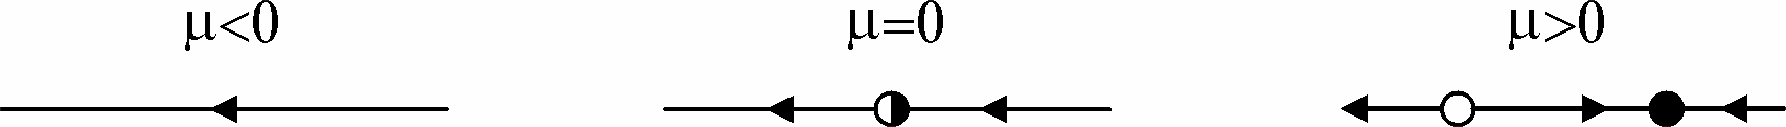
\includegraphics[width=\linewidth]{fig/lect2/5}
 	\caption{Фазовая прямая системы \eqref{eq:2.10} для различных значений параметра $\mu$ }
 	\label{fig:2.5}
 \end{figure} 

 Представленны на рисунках \ref{fig:2.5}-\ref{fig:2.4} результаты удобно представить в виде так называемых бифуркационных диаграмм, представляющих собой зависимость стационарных состояний системы от параметра $\mu$ , который принято называть контрольным параметром. Эти диаграммы для систем \eqref{eq:2.9}-\eqref{eq:2.10} изображены на рис.\ref{fig:2.6}a и b соответственно.

 \begin{figure}[h!]
 	\centering
 	\begin{minipage}{0.49\linewidth}
 		\centering
 		
\includegraphics[]{fig/lect2/6a}

 		(a)
 		\label{fig:2.6a}
 	\end{minipage}
 	\hfill
 	\begin{minipage}{0.49\linewidth}
 		\centering
 		
\includegraphics[]{fig/lect2/6b}

 		(b)
 		\label{fig:2.6b}
 	\end{minipage}
 	\caption{ (a) Бифуркационные диаграммы системы \eqref{eq:2.9} и (b) системы \eqref{eq:2.10}. Пунктирной линией указана ветвь неустойчивых, а сплошной -- устойчивых состояний равновесия}
 	\label{fig:2.6}
 	
 \end{figure}

Таким образом, двукратное равновесия -- негрубое состояние равновесия, которые при сколь угодно малом изменении параметра либо распадается на два грубых, либо исчезает.

\subsection{Понятие о нормальной форме} % (fold)

В определенном смысле системы \eqref{eq:2.9} и \eqref{eq:2.10} описывают все возможные бифуркации двукратных состояний равновесия на прямой и поэтому их называют нормальной формой для этой бифуркации. Другими словами, если какая-либо система прямой имеет двухкратное равновесие, то в окрестности этой точки поведение системы можно описать с помощью уравнения \eqref{eq:2.9} или \eqref{eq:2.10}. Действительно, пусть при $\mu = \mu_0$ система \eqref{eq:2.5} имеет двухкратное равновесия $x=x_0$. Раскладывая правую часть \eqref{eq:2.5} в ряд Тейлора, получим
\begin{gather}
	\dot x = F(x, \mu) = F(x_0, \mu_0)  + (x-x_0) \pdv{F}{x} \eval_{(x_0,\mu_0)} +
	(\mu- \mu_0)\pdv{F}{\mu} \eval_{(x_0,\mu_0)} + \\ 
	\frac12 (x-x_0)^2 \pdv[2]{F}{x} \eval_{(x_0,\mu_0)} + \dots
	\label{eq:2.11}
\end{gather}
Поскольку
\begin{equation}
	\label{eq:}
	F(x_0, \mu_0) = 0, \quad \lambda(\mu_0) = \pdv{F}{x}\eval_{x_0, \mu_0} = 0 ,
\end{equation}

 то \eqref{eq:2.11} можно переписать в следующем виде
 \begin{equation}
 	\label{eq:2.12}
 	\dot x = a(\mu - \mu_0) + b (x-x_0)^2 + \dots ,
 \end{equation}
 где $a = \pdv{F}{x}\eval_{(x_0, \mu_0} $, $b =\frac12 \pdv[2]{F}{x}\eval_{(x_0, \mu_0)}$.
 Очевидно, что уравнение \eqref{eq:2.12} путем введения новых переменных и параметра принимает вид \eqref{eq:2.9} или \eqref{eq:2.10}.
% subsubsection понятие_о_нормальной_форме (end)
\subsection{Транскритическая бифуркация} % (fold)

Существует значительное число задач, в которых число состояний
равновесия при изменении параметров сохраняется, но их устойчивость
меняется. Такая бифуркация носит название транскритической или смены
устойчивости состояния равновесия. Нормальная форма для транскритической
бифуркации задается уравнением
\begin{equation}
	\label{eq:2.13}
	\dot x = \mu x -x^2
\end{equation}
или уравнением 
\begin{equation}
	\label{eq:2.14}
	\dot x = \mu x+ x^2	
\end{equation}

Динамика уравнений \eqref{eq:2.13}, \eqref{eq:2.14} в зависимости от управляющего параметра $\mu$ представлена на рис.\ref{fig:2.7}a и \ref{fig:2.7}b соответственно

\begin{figure}[h!]
	\centering
	\begin{minipage}{0.49\linewidth}
		\centering
		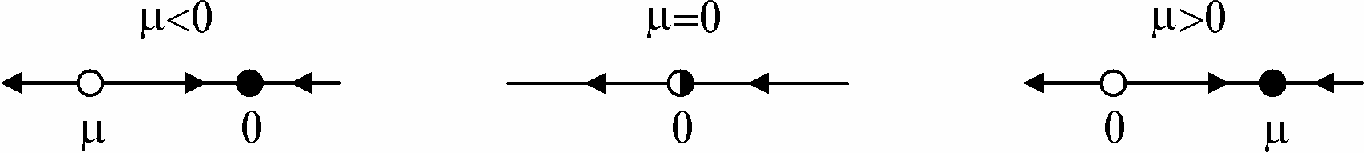
\includegraphics[]{fig/lect2/7a}

		(a)
		\label{fig:2_7a}
	\end{minipage}
	\vfill
	\begin{minipage}{0.49\linewidth}
		\centering
        
\includegraphics[]{fig/lect2/7b}

		(b)
		\label{fig:2_7b}
	\end{minipage}
	\caption{Разбиение фазовой прямой на траектории для системы \eqref{eq:2.13} и \eqref{eq:2.14} соответственно}.
	\label{fig:2.7}
\end{figure}

Принимая во внимание рузультаты представленные на рис.\ref{eq:2.7}, устанавливаем вид буфурцационных диаграмм для систем \eqref{eq:2.13} и \eqref{eq:2.14} (см. рис.\ref{fig:2.8})  
\begin{figure}[h!]
	\centering
	\begin{minipage}{0.49\linewidth}
		\centering
		
\includegraphics[]{fig/lect2/8a}

		(a)
		\label{fig:2_8a}
	\end{minipage}
	\hfill
	\begin{minipage}{0.49\linewidth}
		\centering
		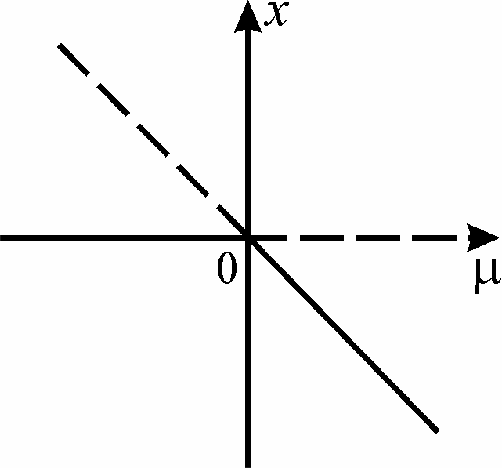
\includegraphics[]{fig/lect2/8b}
        
		(b)
		\label{fig:2_8b}
	\end{minipage}
	\caption{Бифуркационные диаграммы системы \eqref{eq:2.13} (a) и системы \eqref{eq:2.14} (b). Ветвь устойчивых состояний равновесия отмечена сплошной лнией, а неустойчивых -- пунктирной.}
	\label{fig:2.8}
	
\end{figure}
% subsubsection транскритическая_бифуркация (end)

\subsection{Трехкратное равновесие} % (fold)

Эта бифуркация типична для систем, обладающих симметрией.
Например, многие физические задачи имею пространственную симметрию
между левым и правым направлениями. В таких системах состояния
равновесия рождаются и исчезают парами. Нормальная форма бифуркации
трехкратное равновесие определяется уравнениями

\begin{equation}
	\label{eq:2.15}
	\dot x = \mu x - x^3,
\end{equation}
\begin{equation}
	\label{eq:2.16}
	\dot x = \mu x + x^3. 
\end{equation}

Нетрудно видеть, что уравнения \eqref{eq:2.15} и \eqref{eq:2.16} инвариантны относительно
преобразования $x \rightarrow -x$. Исследование динамики уравнения \eqref{eq:2.15} представлено
на рис.\ref{fig:2.9}.

\begin{figure}[h!]
	\centering
	
\includegraphics[width=\linewidth]{fig/lect2/9}
	\caption{Разбиение фазовой прямой на траектории для системы \eqref{eq:2.15} при различных значениях параметра $\mu$}
	\label{fig:2.9}
\end{figure}


Обратим внимание на то, что в момент бифуркации, т.е. при $\mu=0$, ляпуновский характеристический показатель $\lambda(0) = 0$ , а само состояние равновесия, несмотря на это является устойчивым. Исследование уравнения \eqref{eq:2.16} проводится аналогично предыдущему и мы предлагаем читателю провести его самостоятельно. Представим здесь лишь соответствующую бифуркационную диаграмму (см.рис. \ref{fig:2.10}b).
\begin{figure}[h!]
    \centering
    \begin{minipage}{0.45\linewidth}
            \centering
            
\includegraphics[]{fig/lect2/10a}

            (a)
    \end{minipage}
    \begin{minipage}{0.45\linewidth}
            \centering
            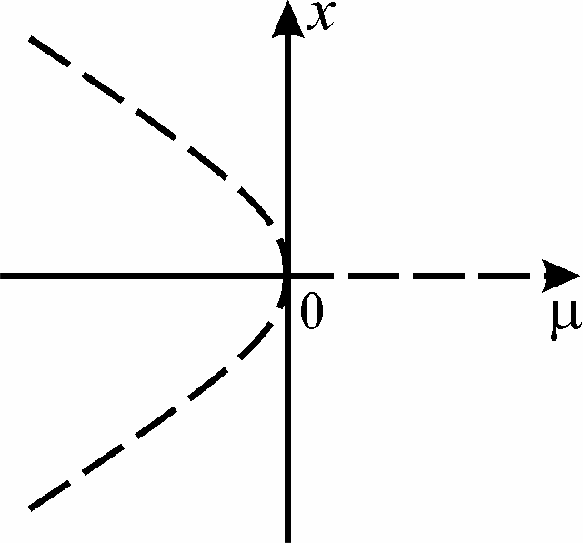
\includegraphics[]{fig/lect2/10b}

            (b)
    \end{minipage}
        \caption{Буфуркационные диаграммы системы \eqref{eq:2.15}(а) и системы \eqref{eq:2.16}(b).
    Ветвь устойчивых состояний равновесия отмечена сплошной линией, а неустойчивых -- пунктирной.}
    \label{fig:2.10}
\end{figure}
% subsubsection трехкратное_равновесие (end)
% subsection бифуркации_состояний_равновесия (end)
\section{Система на окружности}%
\begin{figure}[h]
        \centering
        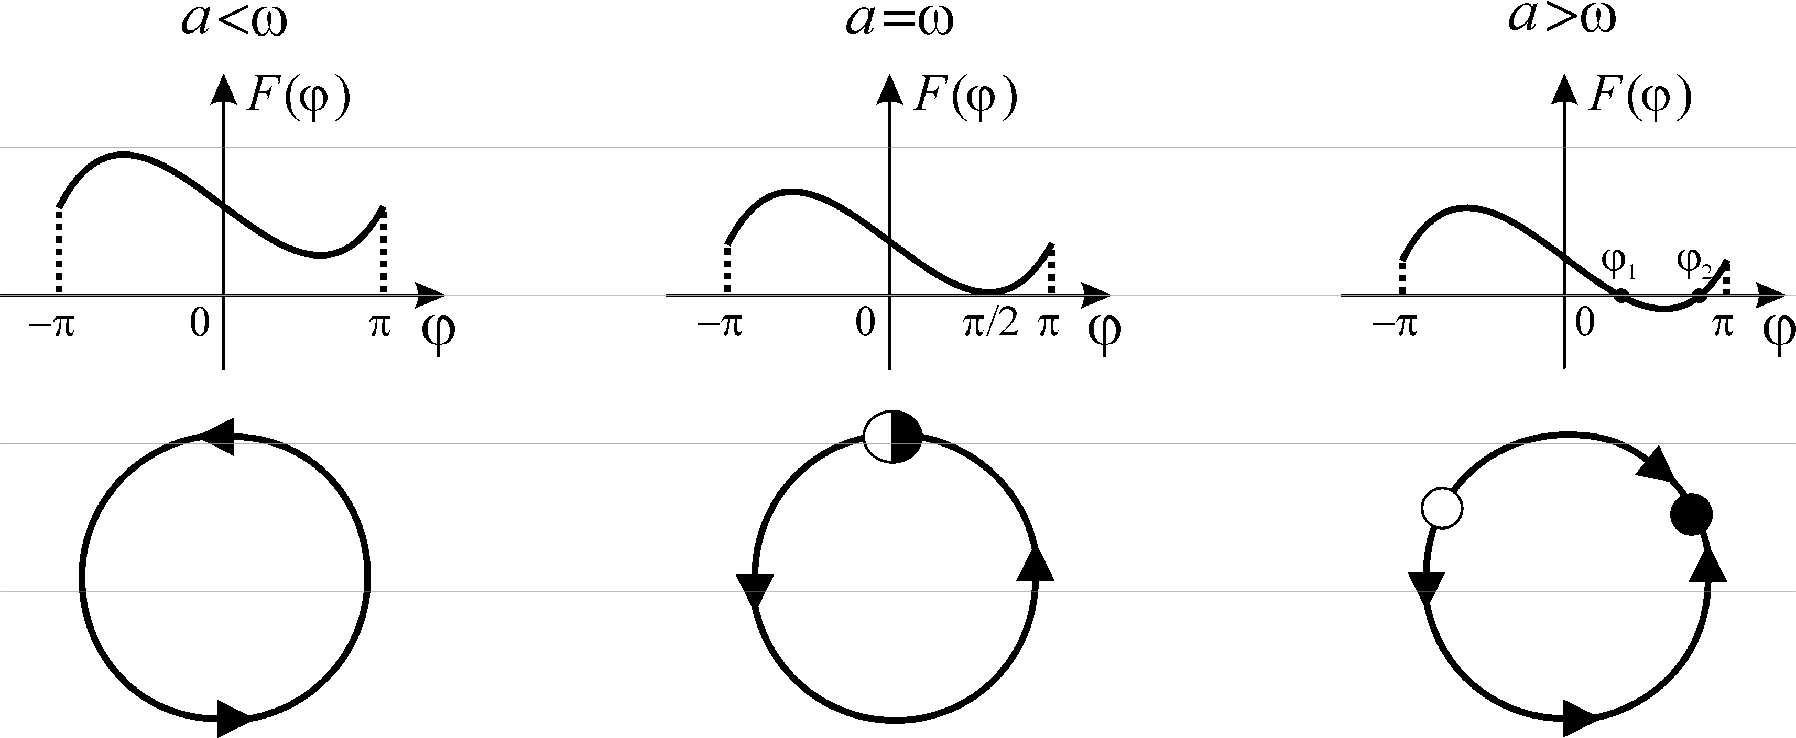
\includegraphics[width=\linewidth]{fig/lect2/11}
        \caption{Разбиение окружности $S_1$ на траектории для различных значений параметра $a$.}
        \label{fig:2.11}
\end{figure}

Рассмотрим  уравнение первого порядка следующего вида
\begin{equation}
    \label{eq:2.17}
    \dot \phi = F(\phi) , \text{ где } F( \phi + 2 \pi) = F( \phi ) 
\end{equation}
Уравнения такого вида возникают при описании динамики реальных систем, у которых переменная состояния изменяется циклически. Например, простейшая безфильтровая система фазовой автоподстройки (см. лекцию 4, уравнение \eqref{eq:4.23}) описывается уравнением $\dot \phi + \sin \phi = \gamma$. В силу периодичности правой части \eqref{eq:2.17} по $\phi$ её фазовым пространством является окружностью $S^1$. Поясним основные свойства таких систем на следующем примере. Рассмотрим уранение
\begin{equation}
    \label{eq:2.18}
    \dot \phi = \omega - a \sin \phi   , 
\end{equation}
где $a$ и $ \omega$ -- параметры, $a\geq0$, $\omega=0$ . При $a=0$ общее решение уравнения \eqref{eq:2.17} имеет вид
\begin{equation}
    \label{eq:}
    \phi = \omega t + \phi_0, \quad \phi_0= \const
\end{equation}
и описывает равномерное вращение изображающей точки по окружности $S^1$. Исследование системы \eqref{eq:2.18} образуется двукратное равновесие, которое при изменении параметров либо распадается на два грубых $(a > \omega)$ либо исчезает  $(a<\omega)$ в \eqref{eq:2.18} происходят вращательные движения, однако эти движения, однако эти движения неравномерны, поскольку скорость $\dot \phi$ не является постоянной (наибольшая скорость достигается при $\phi = - \frac{\pi}{2},$ а минимальная при  $\phi = \frac{\pi}{2}$ ). При $a>\omega$ на окружности $S^1$ существует два грубых состояния равновесия: $\phi = \phi_1 = \arcsin(\omega/a)$ и $\phi = \phi_2= \pi - \arcsin(\omega/a)$. Состояние равновесия $\phi=\phi_1$ -- устойчивое, а $\phi = \phi_2$ -- неустойчивое.

